\newpage
\begin{center}
	\textbf{\large 2. МЕТОД РАСЧЕТА}
\end{center}

\refstepcounter{chapter}
\addcontentsline{toc}{chapter}{2. МЕТОД РАСЧЕТ}

Для нахождения аннигиляционных потоков нужно решить уравнение больцмана для 
эволюции частиц темной материи внутри солнца.

В уравнении больцмана правая чать --- интеграл столкновений, 
который описывает изменение распределений при определенных видах столкновений.
В общем случае его величина выражается при помощи матричного элемента \\
$N$-частичного столкновения.

\tikzstyle{vertex}=[auto=left,circle,fill=black!25,minimum size=20pt,inner sep=10pt]
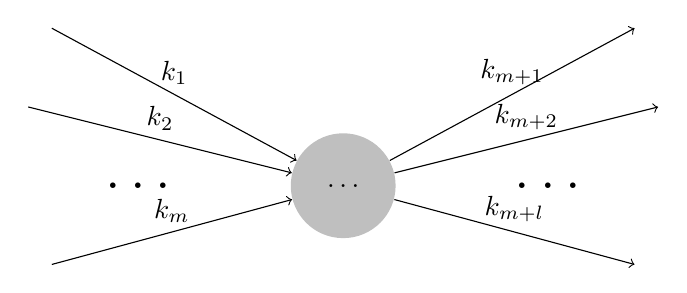
\begin{tikzpicture}
	
	\node[vertex] (sc) at (4,0) {$\dots$};
	
	\draw[->] (0.3,2)--(sc) node [midway, above] {$k_1$};
	\draw[->] (0,1)--(sc) node [midway, above] {$k_2$};
	\draw[->] (0.3,-1)--(sc) node [midway, above] {$k_m$};
	
	\path (1.4,0.6) -- (1.4,-0.6)  node [font=\huge,midway]{$\dots$};
	
	
	\draw[->] (sc)--(8-0.3,2) node [midway, above] {$k_{m+1}$};
	\draw[->] (sc)--(8,1) node [midway, above] {$k_{m+2}$};
	\draw[->] (sc)--(8-0.3,-1) node [midway, above] {$k_{m+l}$};
	
	\path (6.6,0.6) -- (6.6,-0.6)  node [font=\huge, midway]{$\dots$};
\end{tikzpicture}

\begin{equation}
	\label{st_common}
	\frac{dN}{dt} = \frac{P}{T} = \int d^3\vec{r} \prod_{i \in in,out} \cfrac{d^3\vec{k}_i}{2 E_i (2\pi)^3} |\mathcal{M}|^2 (2\pi)^4 \delta^{(4)}(k_{out} - k_{in}) \prod_{i \in in} f_B(\vec{r},\vec{k}_i)
\end{equation}

где $\mathcal{M}$ ---  матричный элемент процесса в релятивисткой нормировке,
$f_B(\vec{r},\vec{k}_i)$ --- функции распределения частиц по координате и импульсу.

Этот интеграл будет фигурировать в соотношениях захвата, матрицы соударений и аннигиляции.

%%%%%%%%%%%%%%%%%%%%%%%%%%%%%%%%%%%%%%%%
%CAPTURE%CAPTURE%CAPTURE%CAPTURE%%%%%%%%
%%%%%%%%%%%%%%%%%%%%%%%%%%%%%%%%%%%%%%%%
\section{Расчет числа захваченных частиц}

Для нахождения числа захваченных частиц необходимо найти плотности частиц
темной материи в каждой точке небесного тела. Предполагая изотропность 
сферического тела, можно найти решение стационарного уравнения Больцмана как функцию от 
первых интегралов движения --- энергии и момента импульса (на единицу массы).

\begin{equation}
	\label{boltsman_capt}
	\tderiv{f(\vec{v},\vec{r})} = \deriv{f}{t}+
	\deriv{f}{\vec{r}}v - \deriv{f}{\vec{r}}\nabla\phi(r)
\end{equation}


\begin{equation}
	%\label{boltsman_capt}
	f(\vec{v},\vec{r}) = f(u^2,L)
\end{equation}

где 
\begin{eqnarray}
	L = rv \sin {\theta_{nu}}\\
	u^2 = v^2 + \phi(r)
\end{eqnarray}
а $\theta_{nu}$ --- угол между напрвлением скорости и радиус вектором $\vec{r}$ от центра 

Вдали от небесного тела функция распределения ТМ соответствует распределению ТМ
в гало внутри галактики 

\begin{equation}
	%\label{boltsman_capt}
	f(r=\infty,\vec{u}) = n_{\chi}f_{\infty}(u)
\end{equation}



Также, необходимо учесть движение самого небесного тела относительно гало. Поэтому функцию распределения $f_{\infty}(u)$ необходимо выразить исходя из плотности 
заданной в переменной $\vec{\xi} = \vec{u} - \vec{u}_0$. 
Предполагая изотропность распределения ТМ внутри гало, можно найти $f_{\infty}(u)$
путем усреднения $f_{\infty}(\vec{\xi})$ по направлению вектора скорости $\vec{\xi}$.

\begin{equation}
	\xi^2 = (\vec{u} - \vec{u_0})^2 = u^2 + u_0^2 - 2 u u_0 \cos{\theta}
\end{equation}

\begin{equation}
	f_{\infty}(u) =
	 \int_{-1}^{1} f\left(\sqrt{u^2+u_0^2-2u_0 u \cos{\theta}}\right)
	 d \cos{\theta}
\end{equation}

При усреднени плотности ТМ по углам сферы пропадает зависимость от момента импульса.
Тогда выраженное с помощью переменной $u$ распределение частиц в гало \ref{dens_infty_xi} будет следующим:

\begin{equation}
	\label{dens_infty_u}
	f_{\infty}(u)  = 
	\cfrac{e^{-\frac{(u-u_0)}{2\xi_0^2}}}{(2\pi\xi_0^2)^{\frac{3}{2}}}
	\cfrac{1-e^{-\frac{2u u_0}{\xi^2}}}{\frac{2u u_0}{\xi^2}}
\end{equation}

Эта функция распределения будет находится в интеграле столкновений для скорости захвата. 
Для вычисления скороти захвата необходимо учесть столкновения с каждым сортом частиц
(мы будем учитывать столкновения на ядрах элементов).

\begin{equation}
	\label{capture_rate}
	C_{+} = {\int{d^{3}\vec{r} \cdot d^{3}\vec{v}f_{k}\left( {r,v} \right) \cdot n_{i}f_{B}\left( {\vec{v}}_{1} \right)d^{3}{\vec{v}}_{1} \cdot 	
	\Gamma_{с}\left( \vec{v},{\vec{v}}_{1},r \right)}}
\end{equation}
где $\Gamma_{с}$ --- это сечение соударения умноженное на скорость
\begin{equation*}
	\label{eq:Gamma_def}
	\Gamma_{с}\left( {\vec{v},{\vec{v}}_{1},r} \right) = {\int\limits_{v' < v_{esc}}{d^{3}{\vec{v}}\,'\delta\left( {E_{f} - E_{in}} \right) \cdot \cfrac{m_{k}^{3}\left| \mathcal{M} \right|^{2}}{64\pi^{2}m_{i}^{2}m_{k}^{2}}}}
\end{equation*}

В интеграле $n_{i}f_{B}(\vec{v}_1)$ --- это концентрация 
$i$-го элемента в теле и больцмановский термальный фактор. Для получения 
концентрации используется файл, где представленны массовые доли элементов в
зависимости от рамдиуса $\widetilde{\rho}_i(r)$ 
а также безразмерная (нормированная на единицу) плотность в зависимости от радиуса.
\begin{equation*}
	n_{i}(r) = n_p \widehat{\rho}(r) \widetilde{\rho}_i(r)  \cfrac{m_p}{m_i}
\end{equation*}

Кинематику соударения будем считать в переменных $\vec{V}$ --- скорость центра
масс и $\vec{\nu}$ --- скорость частицы ТМ относительно центра масс

\begin{align}
	\label{eq:kinematics_cm}
	\vec{V} = \cfrac{m_k \vec{v}_k + m_i \vec{v}_1}{m_k+m_i}\\
	\vec{\nu} = \frac{m_{i}}{m_{i} + m_{k}}\left( {\vec{v} - {\vec{v}}_{1}} \right)
\end{align}
Тогда $\Gamma_{с}$ равна следующему интегралу
\begin{equation}
	\Gamma_{с}\left( {\vec{v},{\vec{v}}_{1},r} \right) = \cfrac{m_{i}}{m_{k}\left( m_{i} + m_{k} \right)}4\pi\nu'd\vec{n}\,' \cdot \cfrac{m_{k}^{3}\left| \mathcal{M} \right|^{2}}{64\pi^{2}m_{i}^{2}m_{k}^{2}}
\end{equation}
причем интеграл по телесному углу $d\vec{n}\,'$ ведется только в той области, которая соответствует захвату, то есть $v' = |\vec{V} + \vec{\nu}\,'| < v_{esc}(r)$, где $v_{esc}(r)$ ---
скорость "выхода" \space из гравитационной ямы, порождаемой небесным телом, при удалении от центра на расстояние $r$.

Расчет этого интеграла проводится методом Монте-Карло. Для этого 
каждая величина в интеграле (скорости, радиус) вычисляется с помощью генератора 
псевдослучайных чисел, а в итоговый интеграл прибавляется произведение дифференциалов.

Так, радус можно определить как $r = r_{\odot}(g())^{\alpha}$, 
где $g()$ --- значение генератора случайных чисел от 0 до 1, $r_{\odot}$ --- радиус небесного тела, а $\alpha$ --- 
положительное число, определяющее, насколько близко к центру будут генерироваться 
события. Тогда $d^3r = 4\pi r^2dr = V \cdot 3 \alpha r_{nd}^{\frac{3\alpha-1}{\alpha}}$.
$r_{nd}$ --- безразмерный радиус.

Величина $f_{B}\left( {\vec{v}}_{1} \right)d^{3}{\vec{v}}_{1}$ в интеграле 
соответствует генерации термальной скорости ядра.

При интегрировании по функции распределения частиц ТМ $d^{3}\vec{v}f_{k}$ берется
известное из \ref{dens_infty_u} распределение, причем $v^2 = u^2 - \varphi(r)$. Тогда 
этот фактор в интеграле равен  $n_{\chi} 2\pi v du^2 f_{\infty}(u)$, который можно просто получить с помощью двумерного распределения гаусса для величины $u$.

Для удобства происходит обезразмеривание интеграла путем выноса из него размерных констант.
В итоге должно получится

\begin{equation}
	\label{capture_simple}
	C_+ = Vn_{\chi} \cdot \sigma_{0} n_p v_{esc} \cdot c_+
\end{equation}

%где $V$ --- объем небесного тела, $n_{\chi}$ --- концентрация частиц ТМ в гало,
%$n_p$ --- средняя концентрация проонов в небесном теле 
%(равна массе тела деленной на объем и массу протона), $v_{esc}$ --- скорость выхода на поверхности небесного тела. %В качестве  $\sigma_0$ мы возмем следующую величину:


Безразмерное отношение $\left| \mathcal{M} \right|^{2}/
\left| \mathcal{M}_0 \right|^{2}$ обозначим как $\Phi \cdot dF$, где $\Phi$ --- отвечает за когерентное рассеяние и для спин-независимого взаимодействия равен $A^4$, а $dF$ --- форм фактор, возникающий из-за размеров ядра.
\begin{equation}
\begin{split}
	\label{capture_nd}
	c_+ = \sum_i \int [3r_{nd}^2d r_{nd}]
	\cdot[d^3\vec{v} f_k(r,v)] \cdot 
	\widehat{\rho}(r) \widetilde{\rho}_i(r) 
	\cdot[f_{B}(\vec{v}_1) d^3\vec{v}_1] \cdot\\ 
	\cdot\cfrac{\nu'}{v_{esc}} d\vec{n}\,' \cdot
	\cfrac{m_{p} (m_p+m_k)^2}{m_i^2 ( m_i + m_k)}
	\cdot \Phi \cdot dF
\end{split}
\end{equation}

\section{Расчет распределения частиц}

Вся информация о распределении частиц в фазовом объеме $d\Phi = d^{3}\vec{x}d^{3}\vec{v}$
требует знания распределения частиц в 6 измерениях. Для упрощения задачи используется
предположение об однородности задачи. В таком случае число переменных может быть сведено 
до 3х: радиус $r$, скорость в направлении радиуса $v_r$ и момент ипмульса $L = r v_{\tau}$.
Фазовый объем в тих переменных будет $d\Phi = 8\pi^{2}drdv_{r}dL^{2}$. Решая в этих
координатах уравнение движения можно сменить переменные на энергию $E$, момент 
импульса $L$ и время $\tau$(имеется ввиду не настоящее время, а временная координата точек на траектории с определенными энергией и моментом импульса). От последней переменной можно
избавиться путем усреднения по траэктории. Тогда левая часть уравнения Больцмана станет
частной производной функции распределения по времени, а правая --- усреднением интеграла столновения по траектории за период траектории. Итоговое уравнение должно принять вид:
\begin{equation}
	\label{eq:boltsman_EL}
	\deriv{f(E,L)}{t} = C\left( {E,L} \right) + St\lbrack f\rbrack(E,L)
\end{equation}
Такое допущение возможно, если при движении фазового объема вдоль траектории число 
частиц в нем не успевает существенно измениться. То есть вероятность столкновения частицы,
которая по порядку величины составляет $\sigma_0 n_p R_{\odot}$ должна быть малой величиной. При интересующих нас сечениях ($\sigma_0 \approx 10^{-42} cm$) эта величина 
имеет порядок $10^{-9}$, что говорит о верности предположения.

Движение в сферическом потенциале $\phi(r)$ в переменных $r$, $v_r$ описывается гамильтонианом (энергией)
\begin{equation}
	\label{eq:move_hamiltonian}	
	E = H = \frac{v_{r}^{2}}{2} + \left( {\phi(r) + \frac{L^{2}}{2r^{2}}} \right) = \frac{v_{r}^{2}}{2} + U_{eff}(L,r)
\end{equation}
\begin{equation}
	\label{eq:move_equations}
	\begin{cases}
		\dot{r} = \cderiv{H}{v_r}\\
		\dot{v}_r= -\cderiv{H}{r}
	\end{cases}
\end{equation}
При этом фазовый объем такой системы $drdv_r$ выражается через энергию-время (координатное время): $drdv_r = d\tau dE$. Таким образом, фазовый объем в переменных энергия-импульс равен
\begin{equation}
	\label{eq:phase_volume_EL}
	d\Phi = 8\pi^{2}drdv_{r}dL^{2} = 8\pi^{2}T(E,L)dEdL^2
\end{equation}
где $T(E,L)$ --- период траектории.

Для расчета используется змерные параметры: безразмерный радиус $x = r/r_{\odot}$, гравитационный потенциал $\varphi(x) = \phi(r)/\phi(r = r_{\odot})$, который находится из файла с моделью тела, безразмерная скорость $\nu$, нормированная на $v_{esc} = \sqrt{-2\phi(r_{\odot})}$, энергия $e = E/\phi(r_{\odot})$, момент имульса $l = x \nu_{\perp}$ и время $\tau =  t \frac{v_{esc}}{r_{\odot}}$. Фазовый объем выражается через безразерные параметры следующим образом:
\begin{equation}
	\label{eq:phase_volume_nd}
	d\Phi = r_{\odot}^3v_{esc}^3 \cdot 4\pi^{2} d\tau de dl^2
\end{equation}


Решать систему будем с помощью квадратуры, когда находятся $x_{min}$,$x_{max}$ (находится ноль функции  $\sqrt{\varphi(x) -e - \frac{l^{2}}{x^{2}}}$) а потом проводится численное интегрирование 
\begin{equation}
	\tau\left( {e,l} \right) = {\int_{x_{1}}^{x_{2}}\frac{dx}{ \sqrt{\varphi(x) -e - \frac{l^{2}}{x^{2}}}}}
\end{equation}
при этом потенциал на каждом отрезке интерполируется в виде $\varphi = a-bx^2$, тогда
\begin{equation}
	\label{eq:eval_dt}
	d\tau \approx \int_{x}^{x+dx}\frac{dx}{ \sqrt{a-bx^2 -e - \frac{l^{2}}{x^{2}}}} = \Eval{\cfrac{\arcsin\left(
			\cfrac{a-e-2bx^2}{\sqrt{(a-e)^2-4bl^2}}
			\right)}{2\sqrt{b}}}{x}{x+dx}
\end{equation}
а снаружи небесного тела потенциал равен $\varphi(x) = - \frac{1}{x}$ и время
\begin{equation}
	\label{eq:tau_out_eq}
	\tau_{out}\left( {e,l} \right) = {\int_{1}^{x_{2}}\frac{dx}{\sqrt{\frac{1}{x} - e - \frac{l^{2}}{x^{2}}}~}} = \frac{\pi}{2(e)^{\frac{3}{2}}} + \frac{\sqrt{1 - e - l^{2}}}{(e)^{\frac{1}{2}}} - \frac{{\arctg}\left( \frac{- 1 + 2e}{2\sqrt{e}\sqrt{1 - e - l^{2}}} \right)}{2(e)^{\frac{1}{2}}}
\end{equation}

\begin{figure}
	\begin{center}
		\begin{tikzpicture}[scale=1]
			\begin{axis}[
					scale = 1.3,
					xlabel = $r_{nd}$,
					ylabel = $\varphi(r)$
				]
			\addplot[] table[x index=1,y index=2] {data/solar_model.dat};
			\end{axis}
		\end{tikzpicture}
		\label{plot:phi_r}
		\caption{Безразмерный потенциал для Солнца}
	\end{center}	
\end{figure}


При движении в гравитационном поле частица может принимать только определенные значения 
момента импульса $L$, которые находятся в интервале от $0$, когда траектория проходит через центр небесного тела, до $L_{max}(E)$, что соответствует круговой таектории.


Мы разобъем отрезок $[E_{min},E_{max}]$ на $N_e$ частей. Тогда, для каждого 
отрезка разбиения $[E_{i},E_{i+1}]$, мы разобъем отрезок $[0,1]$, который соответствует координате $L/L_{max}(E)$ на $N_l$ частей. Причем
$N_l$ бдет зависеть от индекса $i$. Реальной разбиение по $L$ будет получатьса при умножении на $L_{max}(E)$

\begin{figure}
\begin{center}
\begin{tikzpicture}
	\begin{groupplot}[group style={ group size=1 by 1},
		scale = 1.3 ]
	\nextgroupplot[
					title = $E-L$,
					xlabel = $E_{nd}$,
					ylabel = $L_{nd}$,
					enlargelimits=false,
					axis on top,
				]
		\addplot graphics [
		xmin=-5,xmax=0,
		ymin=0,ymax=1,
		] {data/grid/grid-30-30.png};
	
	\end{groupplot}
\end{tikzpicture}
\label{plot:EL_grid}
\caption{Пример разбиения плоскости $E-L$}
\end{center}	
\end{figure}

Выбор такого разбиения связан с удобством его реализации в функциональных языках программирования.

Для нахождения разбиения захваченных частиц по энергии и импульсу необходимо при интегрировании методом Монте-Карло (\ref{capture_nd}) в каждом столкновении считать $E$ и $L$, прибавляя в соответствующий бин гистограммы вес такого столкновения. В результате
скорость захвата станет векторной величиной и вместо количества частиц $N$ у нас будет
вектор $N_i$ являющийся количеством частиц в бине с номером $i$.

\section{Интеграл столкновений}
Для расчета матрицы столкновений в каждом бине выбирается энергия и момент $E_i$ и $L_i$ (в центре бина) и находится траектория движения частицы. Причем часть траектории проходит внутри тела, а другая часть --- снаружи. Соответствующие времена  будут $T_{in}$ и $T_{out}$. 

В интеграле стокновений для захвата \ref{capture_rate} величина $d^{3}\vec{r} \cdot d^{3}\vec{v}f_{k}(r,v)$ соответствует количеству входящих частиц в элементе фазового объема. Поэтому, исходя из \ref{eq:phase_volume_EL}, этот фактор станет равным $N_{j}dt/T(E_i,L_i)$. Интегрирование по $dt$ методом Монте-Карло нужно лишь равномерно сгенерировать время $t$ на внутренней части траектории (тогда $dt = T_{in} d\tau$). в результате матрица столкновения будет иметь вид:
\begin{equation}
	\label{matrix_simple}
	S_{ij} = \sigma_{0} n_p v_{esc} \cdot s_{ij}
\end{equation}
\begin{equation}
	\begin{split}
	\label{st_nd}
	s_{kj} = \cfrac{T_{in}}{T_{in}+T_{out}} \sum_i \int d\tau \cdot \widehat{\rho}(r) \widetilde{\rho}_i(r) 
		\cdot[f_{B}(\vec{v}_1) d^3\vec{v}_1] \cdot 
		\cfrac{\nu'}{v_{esc}} d\vec{n}\,' \cdot \\
		\cdot \cfrac{m_{p} (m_p+m_k)^2}{m_i^2 ( m_i + m_k)}
		\cdot \Phi \cdot dF
	\end{split}
\end{equation}
При этом часть выходящих частиц при столкновениях испарится. За это будет отвечать член с испарением $e_j$

\section{Аннигиляция}
Аннигиляция определяется аналогичным интегралом столкновения, только вместо ядер мишенью являются сами частицы ТМ. 

\begin{equation}
	\label{eq:ann_st}
	\int{d^3\vec{r} d^3\vec{v}  d^3\vec{v_1} 
		f(\vec{r},\vec{v})f_1(\vec{r},\vec{v_1}) \sigma_{ann} 
		|\vec{v}-\vec{v}_1|}
\end{equation}
Для расчета матрицы аннигиляции так же производится обезразмеривание. для этого выносится фактор $\frac{4\pi}{3}\sigma_{a0}v_{a0}/r_{\odot}^3$ и далее интеграл считается в безразмерных параметрах. Вместо величины $ \sigma_{ann} 
|\vec{v}-\vec{v}_1|$ будем использовать 
\begin{equation}
	\phi_{ann} = \cfrac{\sigma_{ann} |\vec{v}-\vec{v}_1| }{\sigma_{a0}  v_{a0}}
\end{equation}

Чтобы в этом интеграле найти фазовые плотности, необходимо разделить число частиц в бине гистограммы на объем этого бина \ref{eq:phase_volume_EL}
\begin{equation}
	\label{eq:phase_dens}
	f(r) = \cfrac{N_i}{d\Phi}
\end{equation}
Факторы $d^3\vec{v}$ и $d^3\vec{v_1}$ соотвкетствуют интегрированию по скоростям. При этом этот объем выражается через переменные $E$ и $L$.
\begin{equation}
	\label{eq:velocity_dens}
	d^{3}\vec{v} = \cfrac{2\pi vdvdL^{2}}{r\sqrt{r^{2}v^{2} - L^{2}}} d\vec{n} = 
	2\pi dEd\sqrt{v^2-\frac{L^2}{r^2}} d\vec{n}
\end{equation}
Причем, поскольку радиальная скорость $v_r$ и тангенциальная $v_{t}$ фиксированны, для $d\vec{n}$ остается только быбор напавления для тангенсальной скорости. Более того, нас интересует лишь модуль раности скоростей, который равен $\sqrt{v^2 + v_{1}^2 - 2\cdot
(v_{t}v_{t1} cos(\phi-\phi_1) \pm v_{r}v_{r1}))}$. Поэтому для определения разности скоростей нужно лишь сгенерировать случайный угол $\phi-\phi_1$ от $0$ до $\pi$.
Интегрирование по радиусу выполняется генерацией $r$ от $r_{min}$ до $r_{max}$, которые определяются из траекторий соответствующих $E, L$ и $E_1, L1$. Однако, если интервалы $[r_{min}, r_{max}]$ для двух траекторий не пересекаются, то частицы не столкнутся и этот член будет равен нулю.
В результате матрица аннигиляции будет иметь форму
\begin{equation}
	\label{eq:ANN_full}
	A_{ij} = \cfrac{3}{4\pi}\cfrac{\sigma_{a0} v_{a0}}{r_{\odot}^3} a_{ij}
\end{equation}
\begin{equation}
	\label{eq:ann_detail}
	a_{ij} =\cfrac{4\pi}{3} \int{[4\pi r^2dr] \cfrac{d^3vd^3v_1}{d\Phi d\Phi_1}} \phi_{ann}
\end{equation}

Также, мы посчитаем аннигиляцию захваченной ТМ и налетающей из гало. Для этого в \ref{eq:ann_st} вместо фактора $d^3vec{v_1}f1(\vec{r},\vec{v})$ происходит интегрирование по входным скоростиям прилетающих частиц ТМ как это было при захвате. Член связанный с аннигиляцией на налетающих из гало частицах представляет из себя вектор, который обозначим как $A^e_i$
\begin{equation}
	\label{eq:ANN_full}
	A^e_{i} = \sigma_{a0} v_{a0} n_{\chi} a^e_{i}
\end{equation}
\begin{equation}
	\label{eq:ann_full}
	a^e_{i} = \int{[4\pi r^2dr] \cfrac{d^3v}{d\Phi}} [d^3v_1f_1] \phi_{ann}
\end{equation} 

\section{Уравнение эволюции}

Эволюция захваченных частиц имеет следующий вид:

\begin{equation}
	\tderiv{N_i} = C_i + S_{ij}N_j - E_i N_i - N_i A_{ij} N_j - A^e_{i}N_i
\end{equation}
где $C_i$ --- захват,  $S_{ij}$ --- матрица рассеяния, $E_i$ -- испарение, $A_{ij}$ и $A^e_{i}$ --- аннигиляция.

В результате обезразмеривания (с учетом \ref{capture_simple}, \ref{st_nd}, \ref{eq:ann_full}) уравнение будет иметь вид:
\begin{equation*}
\begin{split}
	\tderiv{N_i} = V_{\odot}n_{\chi} \cdot \sigma_{0} n_p v_{esc} \cdot c_{i} + \sigma_{0} n_p v_{esc} \cdot (s_{ij}N_j - e_i N_i) -\\
	-\cfrac{3}{4\pi}\cfrac{\sigma_{a0} v_{a0}}{r_{\odot}^3} a_{ij} N_j N_i-
	\sigma_{a0} v_{a0} n_{\chi} \cdot a^e_i N_i
\end{split}
\end{equation*}

Обозначим величину $\sigma_{0} n_p v_{esc}$ как $T_s^{-1}$, которая по порядку величины соответствует вероятности соударения в единицу времени, а величину $V_{\odot}n_{\chi}$ как $N_{\odot}$, по порядку величины равная числу прилетающих частиц ТМ изгало в небесном теле.
Таким образом, разделив на $N_{\odot}$ и умножив на $T_s$, мы получим
\begin{equation}
	\label{eq:evol_compt}
	T_s\tderiv{}\frac{N_i}{N_{\odot}} = c_{i} + \left(s_{ij} \frac{N_j}{N_{\odot}} - e_i \frac{N_i}{N_{\odot}}\right) - a_{\gamma} a_{ij} \frac{N_i}{N_{\odot}} \frac{N_j}{N_{\odot}} -  a^e_{\gamma} a^e_i N_i
\end{equation}
а число $a^e_{\gamma}$ равно $a_{\gamma}$

В программе мы будем использовать безразмерное время $\frac{t}{T_s} \rightarrow t$ и относительное количество частиц $\frac{N}{N_{\odot}}\rightarrow x$. 


\section{Численное решение уравнений эволюции}

Уравнение \ref{eq:evol_compt} состоит из линейной части и нелинейной. Линейная чать отвечает за термализацию и захват и на начальных этапах эволюции преобладает. Линейное уравнение в безразмерных координатах будет иметь следующий вид

\begin{equation}
	\label{eq:evol_x}
	\tderiv{x_i}  = c_{i} + s_{ij} x_j
\end{equation}

Точное решение этого уравнения записывается через матричную экспоненту 
\begin{equation}
	\label{eq:evol_solve}
	\tderiv{x_i}  = x_i(t_0) + \int_{t_0}^{t}{\exp{(s (t'-t_0))}_{ij}c_{j}dt'}
\end{equation}

Физический смысл этого решения заключается в том, что в момент времени $t-t'+t_0$ захватывается $c_i dt'$ частиц в каждом бине, и эти частицы эволюционируют от времени захвата до текущего времени $t$, давая вклад в общее число частиц равный $\exp{(s (t'-t_0))}_{ij}c_{j}dt'$. 

Мы будем приближать матричную экспоненту на некотором интервале $\tau$, используя приближенные методы. 
В первом порядке по $\tau$ получится схема Эйлера. Матрица перехода в этом случае равна

\begin{equation}
	\label{eq:R_tau_euler}
	R(\tau) = 1 + \tau s
\end{equation}

Чтобы решение было корректно, матрица $R(\tau)$ не должна приводить к отрицательному числу чатиц. Для этого $\tau$ должен быть таким, для которого $R(\tau)$ --- неотрицательна. Поскольку матрица $s$ имеет следующий вид 

\begin{equation*}
	\label{s_matrix_view}
	s = \begin{pmatrix}
		-s_{21}-...-s_{n1}-e_1 & s_{12} & \cdots & s_{1n} \\
		s_{21} & -s_{12}-... - s_{n2}-e_2 & \cdots & s_{2n} \\
		\vdots & \vdots & \ddots & \vdots \\
		s_{n1} & s_{n2} & \cdots & -s_{1n}-... - s_{n-1n}-e_n
	\end{pmatrix}
\end{equation*}

где все внедиагональные элементы $s_i$ являются положительными вероятности перейти из одного состояния в другое, а на диагонаяле находятся отрицательные полные вероятности частицы сменить бин, неотрицательность 
$R(\tau)$ достигается при $\tau  \le \tau_{max}$, где

\begin{equation}
	\label{eq:tau_max}
	\tau_{max} = \cfrac{1}{\max_i{s_{ii}}}
\end{equation}

Более того, при таком выборе $\tau$ матрица $R(\tau)$ будет переводить открытое множество возможных конфигураций
$\{\vec{x} \in \mathbb{R}^n | x_i > 0 и \sum_i{x_i} < \epsilon \}$ в себя. Следовательно, собственные значения $R(\tau)$ по модулю меньше единиы для всех $\tau$ меньших $\tau_{max}$ и схема является устойчивой. То есть если $\lambda$ --- собственное значение $s$, то оно удовлетворяет уравнению

\begin{equation}
	\label{eq:lambda_constrains}
	|1+\tau_{max}\lambda| \le 1
\end{equation}

Для того, чтобы увеличть шаг и не потерять устойчивость, необходимо использовать неявную схему. При этом для схемы порядка $n$ погрешность в показателе экспоненты будет равной $\alpha (\tau \lambda)^{n+1} \frac{T}{\tau}$, где $T$ --- конечное время. Если эта погрешность не удовлетворяет требуемой точности $\delta$, то соответствующее решеие доолжно экспоненциально убывать с требуемым показателени экспоненты $-\Re{\lambda} T > N_e$. Так как из \ref{eq:lambda_constrains} следует, что $-\Re{\lambda} > \tau_{max} |\lambda|^2$, можно получить следующее ограничение на $\tau$:

\begin{equation}
	\label{eq:tau_constrains}
	\tau \le \tau_{max}\cdot \left(\cfrac{T}{\tau_{max}}\right)^\frac{n-1}{2n}\cdot 
	\left(\cfrac{1}{N_e}\right)^{\frac{n+1}{2n}}\cdot  \left(\cfrac{\delta}{\alpha}\right)^{\frac{1}{n}}
\end{equation}

Получив оператор эволюции $R(\tau)$ с требуемой точностью, мы будем итерационно умножать его на столбец $\vec{y}$, получая тем самым решение для термализации захваченной порции частиц ТМ.

\begin{equation}
	\label{eq:solver_y}
	\begin{cases}
		\vec{y}_{k+1} = R(\tau) \vec{y}_k\\
		\vec{y}_0 = \vec{c}
	\end{cases}
\end{equation}

Для получения решения $\vec{x}$, мы аппроксимируем интеграл $\ref{eq:evol_x}$ взятый в пределах $[t,t+\tau]$ матрицей $I(\tau)$, тогда

\begin{equation}
	\label{eq:solver_x}
	\vec{x}_{k+1} = \vec{x}_{k} + I(\tau) \vec{y}_k
\end{equation}
Для второго порядка интегрирования можно взять
\begin{equation}
	\label{eq:I_tau}
	I(\tau) = \cfrac{1+R(\tau)}{2}
\end{equation}

Тогда если число шагов равно $m$ а размер пространства равен $N$, то сложность вычисления будет $O(mN^2)$.
Можно потенциально ускорить расчет, если пропускать $2^p$ шагов, используя возможность возвести матрицу в степень за логарифмическое влемя. Новый шаг $\tau_p$ тогда будет равен $2^p \tau$, а оператор эволюции 

\begin{equation}
	R_p(\tau_p) = R(\tau)^{2^p}
\end{equation}
Матрица, аппроксимирующая интеграл $I_p(\tau_p)$ тоже вычисляется за логарифмическое время при помощи рекуррентного соотношения
\begin{equation}
	I_p(\tau_p) = I_{p-1}(\tau_{p-1})\cdot (1 + R_{p-1}(\tau_{p-1}))
\end{equation}
В итоге, сложность будет $O(p N^3 + \frac{m}{2^p}N^2)$, что быстрее простого итеративного метода в случае, когда число итераций превышает размер системы.

Для учета аннигиляции мы будем использвать схему первого порядка по $\tau$, умножив матрицу эволюции $R(\tau)$, соответствующую линейному уравнению, на матрицу эволции квадратичного слагаемого:

\begin{equation}
	R_1(\tau) = R(\tau)\cdot R_a(\tau)
\end{equation}
где
\begin{equation}
	R_a(\tau)_{ii} = e^{-\tau\sum_k{a_{ki}x_k}}
\end{equation}

\section{Модификация уравнения для двухкомпонентной темной материи}

Для двухкомпонентная ТМ, состоящей из более легкой фракции (обозначим за $L$) и более тяжелой ($H$), рассматривается еще и распределение по этим состояниям. Индексы, соответствующие легким частицам будут иметь букву $l$, а тяжелые --- букву $h$. Уравнение для величины $x$ будет следующим

\begin{equation}
	\label{eq:evolution_inelastic}
	\begin{cases}
		\tderiv{x_l} = \nu^L c_l + s_{lh} x_h - \sum_h{s_{hl}}x_l - e_l x_l - a_{\gamma}^{L} x_l - a_{\gamma}^{LL} a_{l l'} x_l x_{l'}  - a_{\gamma}^{HL} a_{h' l} x_l x_{h'}\\
		\tderiv{x_h} = \nu^H c_h + s_{hl} x_l - \sum_l{s_{lh}}x_h - e_h x_h - a_{\gamma}^{H} x_h
		- a_{\gamma}^{HH} a_{h h'} x_h x_{h'}  - a_{\gamma}^{HL} a_{h l'} x_{l'} x_{h}\\
	\end{cases}
\end{equation}

Коэффициенты $\nu^L$ и $\nu^H$, стоящие перед вектором захваченных частиц, являются долями частиц в гало, которые дают вклад в соответствующий захват. То есть $\nu^L$ --- это доля тяжелых частиц в гало, а $\nu^H$ --- легких. 

Коэффициенты аннигиляции являются входными параметрами и зависят от сечения аннигиляции легких с легкими, легких с тяжелыми и тяжелых с тяжелыми. При этом, для двухчастичной аннигиляции параметры $a_{\gamma}^{L}$ и $a_{\gamma}^{H}$ должны быть равны:

\begin{equation}
	\label{eq:require_a_gamma}
	\begin{cases}
		a_{\gamma}^{L} = \nu^L a_{\gamma}^{HL} + \nu^H a_{\gamma}^{LL}\\
		a_{\gamma}^{H} = \nu^H a_{\gamma}^{HL} + \nu^L a_{\gamma}^{HH}
	\end{cases}
\end{equation}